\documentclass[10pt,twocolumn,letterpaper]{article}

\usepackage{cvpr}
\usepackage{times}
\usepackage{epsfig}
\usepackage{graphicx}
\usepackage{amsmath}
\usepackage{amssymb}

% Include other packages here, before hyperref.

\usepackage{subcaption}
\usepackage{siunitx}

% If you comment hyperref and then uncomment it, you should delete
% egpaper.aux before re-running latex.  (Or just hit 'q' on the first latex
% run, let it finish, and you should be clear).
\usepackage[pagebackref=true,breaklinks=true,letterpaper=true,colorlinks,bookmarks=false]{hyperref}

\newcommand{\R}{\mathbb{R}}
\newcommand{\A}{\mathcal{A}}
\newcommand{\D}{\mathcal{D}}
\newcommand{\I}{\hat{I}}
\newcommand{\Z}{\mathbb{Z}}
\newcommand{\m}[1]{{\mathrm{\bf #1}}}
\newcommand{\E}{\tilde{\m{I}}}
\newcommand{\F}{\hat{F}}
\newcommand{\lI}{\m{I}}
\newcommand{\mF}{\m{F}}
\newcommand{\bF}{\mathcal{F}}
\newcommand{\J}{\hat{J}}
\newcommand{\lJ}{\m{J}}
\newcommand{\pD}{D^\prime}
\newcommand{\eF}{\hat{\mF}}
\newcommand{\gN}{\m{N}}
\newcommand{\W}{\m{W}}
\newcommand{\M}{\mathcal{M}}
\newcommand{\Pa}{\mathcal{P}}
\newcommand{\pDD}{\D^\prime}
% \cvprfinalcopy % *** Uncomment this line for the final submission

\def\cvprPaperID{****} % *** Enter the EV Paper ID here
\def\httilde{\mbox{\tt\raisebox{-.5ex}{\symbol{126}}}}

% Pages are numbered in submission mode, and unnumbered in camera-ready
\ifcvprfinal\pagestyle{empty}\fi
\begin{document}

%%%%%%%%% TITLE
\title{Learning filters from markers}
\author{Italos Estilon de Souza\\
Institute of Computing - University of Campinas (UNICAMP)\\
Institution1 address\\
{\tt\small italos.souza@ic.unicamp.br}
% For a paper whose authors are all at the same institution,
% omit the following lines up until the closing ``}''.
% Additional authors and addresses can be added with ``\and'',
% just like the second author.
% To save space, use either the email address or home page, not both
\and
Alexandre Falcão\\
{\tt\small afalcao@ic.unicamp.br}
}

\maketitle
%\thispagestyle{empty}

%%%%%%%%% ABSTRACT


%%%%%%%%% BODY TEXT
\section{Introduction}

\section{Preliminaries}

Let $D \subset \Z^d$ for $d > 1$ and let $\m{I}: D \to \R^b$, with $b \ge 1$, be a function that assings to each $p = (x_p, y_q) \in D$ a vector $\m{I}(p) = (I_1(p), I_2(p), \ldots, I_b(p))$.
A multi-band and multi-dimensional image is a pair ${\hat{I} = (D, \m{I})}$. We say that $D$ is the \textit{image domain}, $\m{I}(p)$ is the \textit{local feature vector} of a space element (\textit{spel}) $p \in D$, $b$ is the number of bands, and $d$ is the number of dimensions. In this work, we focus on images with $d=2$. The set of local feature vectors is called \textit{local feature space}.

An adjacency relation $\A \subseteq D \times D$ is a binary relation between spels $p, q \in D$. We focus on reflexive and translation-invariant relations. More precisely, we focus on adjacency relations given by \[\A_{i,j} = \{ (p, q) \in D : \|x_p - x_q\| \le i, \|y_p - y_q\| \le j \}.\] We say that $\A(p) = \{q \in D : (p, q) \in \A\}$ is the set of spels that are adjacent to $p$ with respect to $\A$.

Let $\D$ be a dataset of images that have the same image domain, and let $\lambda(\I) = \{\omega_1, \omega_2, \ldots, \omega_c\}$ be the true label of an image $\I \in \D$ among $c$ classes. A dataset $\D$ is \textit{supervised} if all image $\I \in \D$ is inspected by an expert and she agrees with $\lambda(\I)$. A dataset $\D$ is \textit{unsupervised} if $\lambda(\I) = \emptyset$ for all $\I \in \D$, that is all true labels are unkown. If there exist images with known and unkown true labels, we say that dataset $\D$ is \textit{semi-supervised}.

For a spel $p \in D$ and an adjacency relation $\A$, a \textit{locally expanded feature vector} is given by \[\E(p) = \lI(q_1) \oplus \lI(q_2) \oplus \ldots \oplus \lI(q_{|\A|})\] such as $q_i \in \A(p)$, for $i = 1, \ldots, |\A|$. Observe that for two different spels $p, q \in D$, it might be the case that $|\A(p)| \neq |\A(q)|$.

%resolver a definição de vetor extendido localmente para assegurar que todos os vetores tenham a mesma quantidade de dimensões

A multidimensioal and multi-band filter $\F$ is a pair $(\A, \mF)$ such that $\A \in D \times D$ is a adjacency relation and for all $(p, q) \in \A$, $\mF(p, q)$ assings a vector $(F_1(p, q), F_2(p, q), \ldots, F_b(p, q)) \in \R^b$ with $b \ge 1$ that satisfies the constraint that $\mF(p, q) = \mF(p, q - p)$. We can interpret $\F$ as a moving window that can be placed at any position $p \in D$. We say that $\bF = \{\F_1, \F_2, \ldots, \F_l\}$ is a \textit{filter bank} if for any $\F_i = (\A_i, \mF_i) \in \bF$ and $\F_j = (\A_j, \mF_j) \in \bF$, $\A_i = \A_j$, that is, all filters from $\bF$ has the same adjacency relation.

Now, we define the convolution operation. The convolution between an image $\I = (D, \lI)$ and a filter bank $\bF$ with $m$ filters produces a image $\J = (\pD, \lJ)$, in which, for $p \in \pD$, $\lJ(p) = (J_1(p), J_2(p), \ldots, J_m(p))$, and \[J_i(p) = \sum_{q \in \A(p)}\lI(q) \cdot {\F_i(q - p)},\] for $m = 1, 2,  \ldots, m$.

In convolution neural networks, the filters has the purpose of detecting relevant features. This happens by producing an positive value for spels which have those feaures and negative values for the ones which does not have them. This information is handle by the activation function. An activation function is a pair $\alpha$ that takes an image $\I = (D, \lI)$ as input and produce another image $\hat{A} = (D, \m{A})$ as output.  In this work, we use the \textit{rectified linear unit}, which can be defined as $A_l(p) = \max(0, I_j(p))$, as activation function.

Pooling has the purpose of aggregating nearby information and make convolutinal neural networks less sensible to small variations in data. In this work, we use only max pooling which is a operation that takes an image $\I = (D, \lI)$ with $b$ bands as input and produces an image $\hat{P} = (\pD, \m(P))$ where, for $p \in \pD$, ${\m{P}} (p) = (P_1(p), P_2(p), \ldots, P_b(p))$ such that \[P_i(p) = \max_{q \in \A(p)}{I_i(q)},\] for $i = 1, 2, \ldots, b$, and an adjacency relation $\A$.

When computing the convolution between each image of a dataset $\D$ and each filter of a filter bank, followed by ReLU activation,
at each position $p\in D$, points $\E(p)$ from the
images $\I \in \D$ may be detected at the positive (or
negative) side of a hyperplane with normal vector $\eF_l$ at the origin of $\R^{b \times |\A|}$. The distance
between $\E(p)$ and that hyperplane is proportional to $J_l(p)
=\I(p) \cdot \eF_l$, for $l \in
\{1,2,\ldots,m\}$.

One can then imagine that whenever local patterns $\E(p)$ related to images from different categories appear as
distinct groups of points in $\R^{b\times |\A|}$, they should
be at different sides of the hyperplanes of the filter bank, so
different filters will be able to capture relevant details of distinct
classes. This is precisely the role of the bias in convolutional
neural networks. However, if the center of the points $\E(p)$ is at the origin of $\R^{b\times |\A|}$, the bias
computation becomes unnecessary.

Batch normalization is the operation that places the origin of
$\R^{b\times |\A|}$ at the center of the cloud of points
$\E(p)$, for $p\in D$, from all images $\hat{I}\in
\D$, and then makes those clouds of points for all $p\in D$ so
hyperspherical as possible \cite{ioffe2015batch}. This can be done independently, per
position and band, by transforming each image $\I=(D_I,\lI)$
into an image $\hat{N}=(D_I,{\bf N})$, ${\bf
  N}(p)=(N_1(p),N_2(p),\ldots,N_b(p))\in \R^b$, where
\begin{eqnarray}
  N_j(p) & = & \frac{I_j(p) - \mu_j(p)}{\sigma_j(p)} \\
  \mu_j(p) & = & \frac{1}{|\D|} \sum_{\forall \hat{I}\in \D} I_{j}(p) \\
  \sigma^2_j(p) & = & \frac{1}{|\D|} \sum_{\forall \hat{I}\in \D} \left(I_{j}(p)-\mu_j(p)\right)^2
\end{eqnarray}

A convolutional neural network may consist of a sequence of
convolutional layers followed by a pattern classifier. The
convolutional layers extract features from each input image $\I$
and create a global feature vector $\gN$ at the output of the
extra batch normalization after the last convolutional layer. The
classifier may be a linear Support Vector Machine (SVM) or a
Multi-Layer Perceptron (MLP). When using a MLP, the feature space of $\gN$ has usually
its dimensions reduced by a sequence of fully connected layers before
the decision layer.

For instance, assume that ${\gN}={\gN}^{(0)}\in \R^{m\times |D|}$
and let ${\W}^{(1)}_i \in \R^{m\times |D|}$ be the synaptic weight
vector of each neuron $i=1,2,\ldots,k_1$ in a first fully connected
layer with $k_1$ neurons. The result ${\gN}^{(1)}=(N^{(1)}_1,N^{(1)}_2,\ldots,N^{(1)}_{k_1})\in \R^{k_1}$, as
$k_1 = m\times |D|$, is obtained by $k_1$ doct products with ${\W}^{(1)}_i$, $i=1,2,\ldots,k_1$, followed by activation values, such that
\begin{eqnarray}
  N^{(1)}_i & = & \max\{0,\langle {\gN}^{(0)}, {\W}^{(1)}_i\rangle\}.
\end{eqnarray}

For a sequence of $l$ fully connected layers with $k_1,  k_2, \ldots, k_l$ neurons per layer, the above equation becomes recursive 
\begin{eqnarray}
  N^{(l)}_i & = & \max\{0,\langle {\gN}^{(l-1)}, {\W}^{(l)}_i\rangle\}, 
\end{eqnarray}
$i=1,2,\ldots,k_l$, creating a final feature vector ${\gN}^{(l)}\in
\R^{k_l}$ for classification by a decision layer.

For $c$ categories $\omega_1, \omega_2, \ldots, \omega_c$, the
decision layer consists of $c$ neurons with synaptic weights ${\W}_i\in \R^{k_l}$, $i=1,2,\ldots,c$, such that the input image
$\I$ is assigned to class $\omega_j$, $j\in \{1,2,\ldots,c\}$,
whenever
\begin{eqnarray}
  a_i & = & \max\{0,\langle {\gN}^{(L)}, {\W}_i\rangle\},\\ 
  a_j & = & \max_{i=1,2,\ldots,c}\{ a_i \}.
\end{eqnarray}

Given an image $\I = (D, \lI)$ of a dataset $\D$ such that each image has some category $\omega \in \{1, 2, \ldots, c\}$, a \textit{marker} is a pair $(p, \omega)$ where $p \in D$. We denote by $M(\I)$ a set of markers for image $\I$. For a marker $m = (p, \omega) \in M(\I)$, a \textit{patch} is the locally expanded feauture vector of $p$ with respect to some adjacency relation $\A$. We denote by $P(\I, M, \A)$ the set of patches of an image $\I$ with respect to a set of markers and an adjacency relation.

\section{Related work}

\section{The method}
Our method is based on the idea that the network designer is an expert in the application domain or knows well enough to indicate which are the relevant characteristics of the objects of interest. The designer highlights these regions by placing markers. For each marker, the extended local feature vector is taken. These vectors are clustered and the centers of the clusterizes are used as convolutional layer filters.

Let $\D$ be a dataset of images. The designer puts markers on only a subset of the images, let's say $\pDD \subseteq \D$. That is, she produces for each $\I \in \pDD$ a set of markers $\M(\I)$.  This subset of images, using the information from the markers, is used to create a set of patches \[\Pa(\pDD) = \bigcup_{\I \in \pDD}{P(\I, M, \A)},\] with respect to an adjacency relationship also defined by the designer. In this work, we use only circular adjacency relationships.

Given the set of patches $\Pa(\pDD)$ of the subset of images $\pDD$, we use a clustering algorithm to discover groups of $\Pa(\pDD)$. Each group represents a pattern (or set of patterns) highlighted by the designer through the markers. Since the center of each cluster must be a good representative of the characteristics of the group, we can use the centroid as filters to recognize these patterns in the images of $\D$.

However, for it to work properly, patches and images need to be centered at the origin. For this, we use the information from the patches to calculate the mean and standard deviation per band. If the patches are representative of images of $\pDD$ the mean and standard deviation (per band) of $\Pa$ are very close to the mean and standard deviation (per band) of $\pDD$.

Note that the convolution in a spel $p \in D$ corresponds to the doct product of the locally extended feature vecture and the vector that represents the filter. Thus, let $H$ be a hyperplane orthogonal to the vector of a $\mF$ filter. Thus, let $ H $ be a hyperplane orthogonal to the vector of a $ \mF$ filter. Vectors similar to the vector of filter $\mF$ must fall on the same side of the hyperplane as $\mF$. That is, if the vector $\E(p)$ is on the same side of $H$ as $\mF$, then the doct product between $\E (p)$ and $\mF$ is positive, and is negative otherwise. Thus, the doct product between the center of a cluster and each of the vectors of that cluster must be positive, which implies that the center is a good filter to identify the pattern described by that cluster. In the Figure (fazer a figura) we can see an example.

Since all the patches used to produce the filters are centered around the origin, as well as the images of $\D$, we have that the hyperplanes ortogonal to the filters contain the origin, therefor there is no need for bias.

Each convolutional layer is trained individually, one layer at a time. After the convolution operation, we apply the ReLU function to eliminate negative activations and the max pooling operation to aggregate local information. We preserve the output dimensions of convolutional layers so that we can use the same markers used in the previous layer. The new patches are generated from the convolutional layer output and the whole process is repeated to find the filters of the next layer.

\begin{figure}[t]
  \begin{center}
     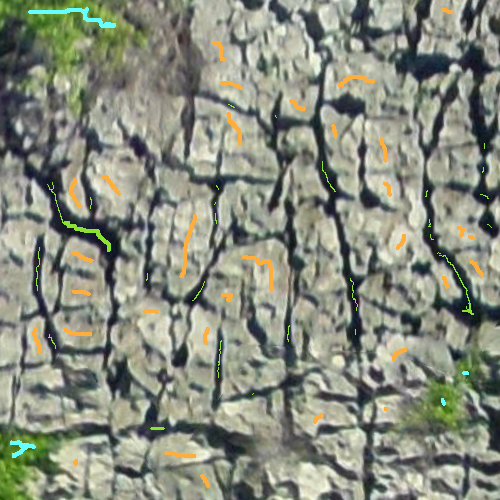
\includegraphics[width=0.8\linewidth]{figures/tile0705-markers.png}
  \end{center}
     \caption{Example of markers.}
  \label{fig:ex-markers}
\end{figure}

To exemplify how our method works, we apply it to the problem of segmenting rock images into vegetation, rock and fractures. In Figure \ref{fig:ex-markers} we can see an example of the markers added by the network designer in regions that she considers relevant to characterize each of the classes.

\begin{figure*}[t]
  \centering
  \begin{subfigure}[b]{0.37\textwidth}
      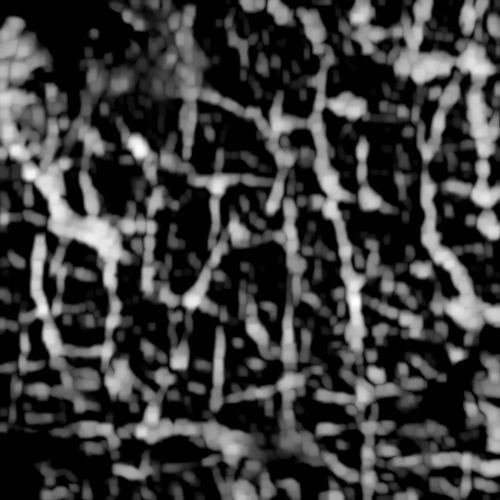
\includegraphics[width=\textwidth]{figures/probabilidade-fratura.png}
      \caption{Probability map for fractures.}
      \label{fig:prob-fractures}
  \end{subfigure}
  ~
  \begin{subfigure}[b]{0.37\textwidth}
      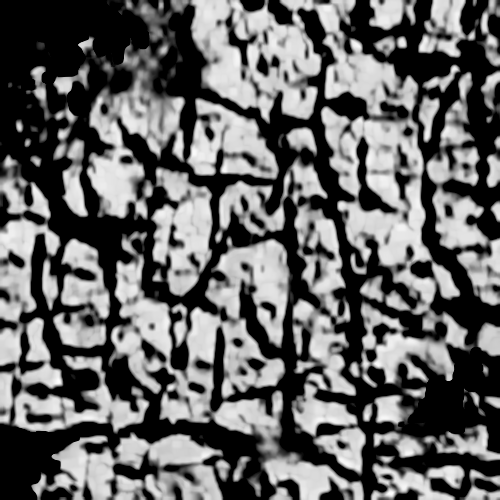
\includegraphics[width=\textwidth]{figures/probabilidade-rocha.png}
      \caption{Probability map for rocks.}
    \label{fig:prob-rocks}
  \end{subfigure}
  ~
  \begin{subfigure}[b]{0.37\textwidth}
      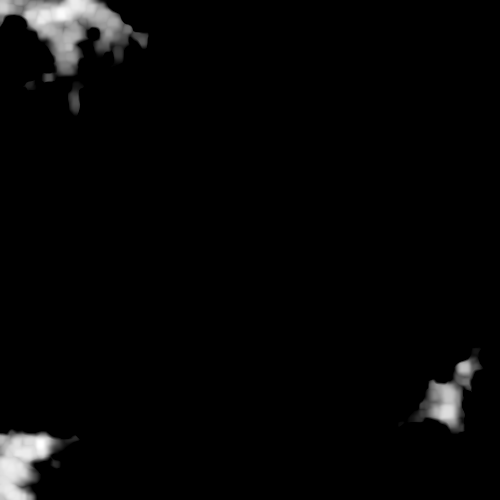
\includegraphics[width=\textwidth]{figures/probabilidade-vegetacao.png}
      \caption{Probability map for vegetation.}
  \label{fig:prob-vegetation}
  \end{subfigure}

  \caption{Probability maps for the classes.}
  \label{fig:prob_map}
\end{figure*}

We designed a neural network with two convolutional layers and used the features extracted by it to produce the probability maps that we can see in Figure \ref{fig:prob_map}, one for each class.

\begin{figure*}[t]
  \centering
  \begin{subfigure}[b]{0.37\textwidth}
    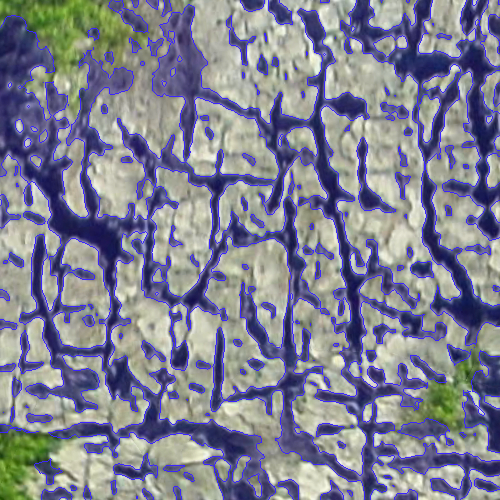
\includegraphics[width=\textwidth]{figures/fratura.png}
    \caption{Segmentation of fractures.}
    \label{fig:segm-fractures}
  \end{subfigure}
  ~
  \begin{subfigure}[b]{0.37\textwidth}
    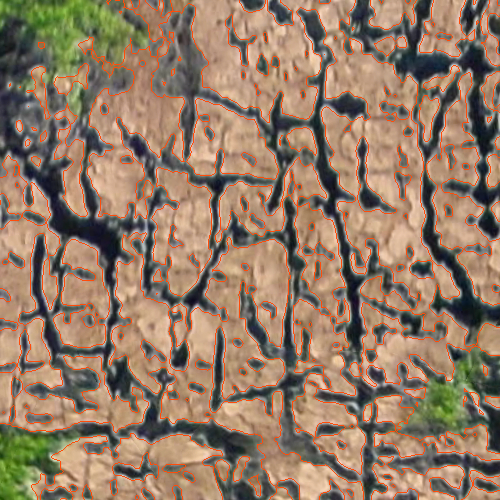
\includegraphics[width=\textwidth]{figures/rocha.png}
    \caption{Segmentation of rocks.}
    \label{fig:segm-rocks}
  \end{subfigure}
  ~
  \begin{subfigure}[b]{0.37\textwidth}
    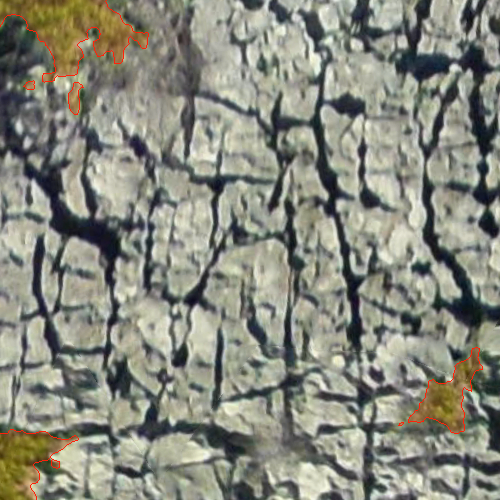
\includegraphics[width=\textwidth]{figures/vegetacao.png}
    \caption{Segmentation of vegetation vegetation.}
  \label{fig:segm-vegetation}
\end{subfigure}

\caption{Segemetation of classes.}
\label{fig:segm}
\end{figure*}

The probability maps were used to produce the segmentations that we can see in Figure \ ref {fig: segm}. For simplify viewing, each image shows the segmentation of one class.

\section{Experiments}
To evaluate our method in a quantitative way, we need a dataset with a ground truth and unfortunately the rock image dataset was not properly labeled.

So, we chose to use a dataset formed from patches of coconut images. The dataset consists of images of dimensions $90 \times 90$ of coconut and non-coconut. The latter class having a large variability. The problem of interest is to classify the images in one of the two classes.

As in reality, labeling images is a costly and time-consuming process, we assume that we only knew the true labels of a small set of samples (one hundred images for each class, totaling two hundred images). That way, we would have only those two hundred images to train any models that we would use to try to solve the problem.

To reduce the impact of chance on the results, we randomly selected three sets of 200 images for training and three sets of 11387 images for testing. We wanted to represent a scenario where the network designer did not have much effort to annotate all these images.

From each of these sets of training images, we selected 4 images using the 2D space projection of the 200 images using the tSNE. We tried to select images that were part of more cohesive groups. Thus, these images are more likely to have characteristics that represent their group.

We placed markers on these images in regions that we consider important to identify the coconut and non-coconut (more diverse) classes. An example of a coconut tree image with markers can be seen in the Figure.

With the markers, we created a convolutional layer with filters of dimensions $7 \times 7$. We did a padding to preserve the dimensions of the images. The network architecture can be seen in the Figure. We used a classifier similar to that of VGG.

For clustering to find the convolutional layer filters, we used K-means to cluster the coconut tree patches in 35 clusters and the non-coconut tree patches in also 35 clusters.

As the experiments were repeated three times, we reported the mean and standard deviation for each of the metrics in the test set. The results can be seen in the Table \ref{tab:results}.

\begin{table*}[h]
  \begin{center}
  \begin{tabular}{|l|c|c|c|}
  \hline
   Method & Precision & Recall & F-score \\
  \hline\hline
  Ours & $0.86 \pm 0.01$ & $0.84 \pm 0.02$ & $0.85 \pm 0.02$\\
  Ours (back) & $0.86 \pm 0.01$ & $0.84 \pm 0.02$ & $0.84 \pm 0.02$\\
  VGG & $0.84 \pm 0.01$ & $0.76 \pm 0.03$ & $0.77 \pm 0.02 $ \\
  VGG (fine tuned) & $0.84 \pm 0.01$ & $0.75 \pm 0.03$ & $0.77 \pm 0.02 $ \\
  \hline
  \end{tabular}
  \end{center}
  \caption{Results.}
  \label{tab:results}
  \end{table*}
  

\section{Conclusions and future work}

{\small
\bibliographystyle{ieee_fullname}
\bibliography{egbib}
}

\end{document}
